%--------------------------------------------------------
% Implementation
%--------------------------------------------------------
\chapter{Implementation}
This chapter will cover the implementation of each three sections of the project as outlined in the requirements and design chapter. It discusses the decisions made for each section and any changes from the design that were made. This chapter will also document any additions made. This chapter will also include the testing process.

\section{Development Approach}

As previously discussed the project should contain 3 separate sections which should be developed prior to the project being implemented under one roof. Therefore, the project utilised an agile development strategy. Agile development allows iterative development where the requirements can change during the development of the project. As agile is used the implementation plan will comprise first implementing the ‘Essential’ sections of the project, these sections can later be revisited and less essential sections can be added.

\subsection{Implementation Plan}

An essential part of any implementation is planning prior to it. As the most important section is the data generation section of the project, this will be done first to ensure that at least some data can be extracted to be used in future sections of the project. The data however must be processed before it can apply to a machine learning model and the data processing will be implemented next. Finally, the data modeling section of the project can be implemented.

To ensure that the project succeeds, any requirement which was given a ‘Essential’ importance in Table \ref{table:req} must be implemented before moving on to the next section. Once all the essential requirements have been implemented, and the project works to a satisfactory level, any remaining requirements given the ‘Important’ importance level can be implemented. Finally, any requirement given the ‘Desirable’ importance level will be implemented, given enough time.
Through this method each part of the project can be split into blocks. When a block of work is complete, its resembles a part of the project which is complete and functioning. 
\subsubsection{Block Plan}
\begin{enumerate}[
    leftmargin=*,
    label={Block \arabic*.},
    ref={Block (\arabic*)}]
    \item Implement all Essential requirements for the Data Generation project section, namely OS.1,OS.4, DG.1-2, DG.4-8. 
    \item Implement all Essential requirements for the Data Processing project section, namely OS.2, DP.1-4. 
    \item Implement all Essential requirements for the Data Modeling project section, namely OS.3, DM.1.
    \item Implement all Important requirements for the project, namely OS.5, DG.3-4, DM.2-3.
    \item Implement other requirements with either a ‘Desirable’ importance or any other requirements not yet implemented.
\end{enumerate}

The project must be done in the order above, ensuring that the project functions correctly at each block and that testing can be done to each block as they are implemented.

\subsection{Programming Language}
The programming language chosen for this project is Python 3.7.4. This is primarily because of my personal familiarity with the language. Coding in a familiar language makes writing code initially easier and also makes debugging code easier. In conclusion, the adoption of a familiar programming language makes programming simpler and quicker.

Python also provides compatibility over a broad variety of operating systems without having to modify the code at all. The code to be written can run on Windows, Unix and Mac satisfying requirement UP.7.

Python also has a large amount of open source libraries to complement the already comprehensive standard library. This means that Python can be moulded with libraries to do a large plethora of things. In this project libraries will launch packer, deal with network data and train a model.

\section{Virtual Machines}
As seen in Figure \ref{fig:vnd} a simple virtual network needs to be automated. This simple network will require an attack machine and a target machine to be generated automatically and connect to the same network, so as to be visible to each other. This will however not represent a usual network, I have made the network simple for prototyping purposes. The same ideas presented here can be altered relatively simply to represent a more complex network with more nodes.

\subsection{Virtual machine images}
To create the virtual machine images, a virtual machine to image must first be created. Creating virtual machines using the VirtualBox GUI is relatively simple, and the process is similar for both systems. An in-depth guide can be seen in the VirtualBox documentation \cite{vb_docs}. 

\subsubsection{Virtual Machine Creation}
Following the step-by-step guide seen in the documentation, the two virtual machines were created. The Kali Linux attack machine was allocated 2GB of RAM and a 20GB Hard Drive, as the machine need not be powerful to execute these basic threats. The Windows 7 target machine was allocated 1GB of RAM and a 32GB Hard drive, the increased hard drive size is because of the space which Windows needs to be installed. The 1GB of RAM should be enough to maintain the operating system as no programs need to be launched during the attack.

Once the machine is launched VirtualBox requests an .iso file to boot from which should contain the relevant files to install an operating system. 

For Kali Linux the .iso file is freely available from their website \cite{kl}. Windows 7 however is not a freely available operating system, therefore a product key was purchased and the .iso file downloaded from their website \cite{w7}. Following the relatively simple step-by-step setup wizards to install both operating systems the machines can now be configured.

\subsubsection{Setting a Static IP}
As discussed in the design section, each virtual machine must have a static local IP address, to allow the attack and target machines to communicate and to allow filtering of packets later on. Altering the static IP address is different for both operating systems. 

\textbf{Kali Linux} - For Kali Linux the static IP can be changed from the command line. First the file  \texttt{/etc/network/interfaces} needs to be altered. Inside that file these lines were added
\begin{verbatim}
    auto eth0
    iface eth0 inet static
    address 192.168.0.14/24
    gateway 192.168.0.1
\end{verbatim}
This alters the ip address of the \texttt{eth0} interface to 192.168.0.14, the ip address which will identify the attack machine. Once this alteration has been made the networking service must be restarted.
\begin{verbatim}
    sudo systemctl restart networking.service
\end{verbatim}
\begin{figure}[h]
    \centering
    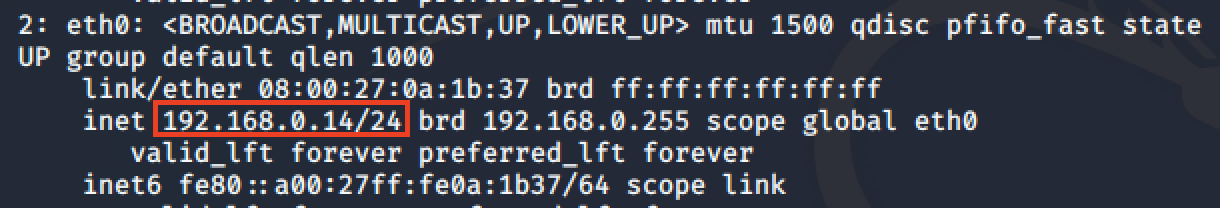
\includegraphics[scale=0.65]{Images/ip.png}
    \caption{IP Configuration for Attack Machine}
    \label{fig:ipfa}
\end{figure}
When the service has restarted, the IP should have changed as in Figure \ref{fig:ipfa}. This IP will stay as the IP address of the machine when the machine will be restarted/exported.

\textbf{Windows 7} - For Windows 7 the static IP can be changed from the Control Panel. First the relevant section of the control panel should be accessed by Start Menu > Control Panel > Network and Sharing Center > Change adapter settings. From here the Local Area Network interface  Internet Protocol Version 4 (TCP/IPv4) properties are accessed, the IP address is then changed to include the static IP address. The static IP for the target machine will be 192.168.0.15. Once saved the IP address of the target machine will have been altered as seen in Figure \ref{fig:ipft}.
\begin{figure}[h]
    \centering
    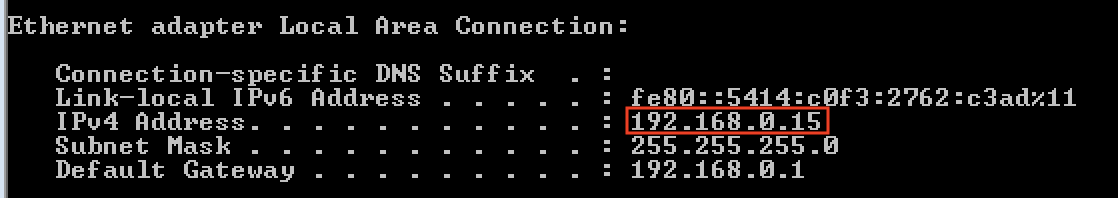
\includegraphics[scale=0.7]{Images/ip7.png}
    \caption{IP Configuration for Target Machine}
    \label{fig:ipft}
\end{figure}

\subsubsection{Target Machine Configuration}
The target machine represents a vulnerable machine which an attacker may take advantage of. As this is the case for the Windows 7 machine the Windows Firewall must be turned off. This can be done by accessing the Windows Firewall section of the Control Panel and turning the windows firewall off. This will allow the machine to become vulnerable to DoS attacks.

\subsubsection{Exporting the Virtual Machines}
Once the machines have been fully configured they must be exported. Virtual machines can be exported to Open Virtualisation Format (OVF) Files via Virtualbox, the full instructions can be found in the Virtualbox documentation \cite{vbovf}. Both the attack and target machines will be exported to OVF files to be used in the project. These images are however rather large, totalling almost 15GB for the two images. This will cause problems if these machines are to be distributed as part of a package.

\subsubsection{Bridged Network Connection}
Setting up a bridged network connection is simple. From the Virtual Machine Settings > Network page the network can be changed from NAT network to a Bridged Network. This involves choosing the interface on the host PC to bridge. 

\subsection{Packer Scripts}
A packer script, as discussed in the design section, is used to build and run a virtual machine from an image. For both the attack machine and target machine a separate JSON script file is needed, and since the attack shell script has to be specified in the provisioners section of the script, this means that each attack will need its own script. To counteract this the name of the attack can be specified on the launching of the program and a python library can alter the attack script.

Packer.py is a library which allows interacting with packer from Python \cite{packerpy}. Once installed the library can be used from within the program to build the template and run the script. Building the template in the program allows many alterations to be made to the script before run-time without writing and saving a new script.

\begin{lstlisting}[language = python]
p = PackerExecutable(self.executable_path)
\end{lstlisting}

Before Packer.py can run the library needs to find the location of the packer executable, without this it cannot run the scripts. Unfortunately the packer executable file is stored in different places depending on computer and operating system. Because of this in the program the user must specify the location of the packer executable. The project will allow the user to specify it within a config file.

\subsubsection{Attack Script}
\begin{lstlisting}[language = python, caption = Attack Script, label=code:atts]
attack_template = """{{
"builders": [
    {{
    "type"                  : "virtualbox-ovf",
    "vboxmanage": [
             ["modifyvm", "{{{{.Name}}}}", "--bridgeadapter1", "{interface}"]
                   ],
    "source_path"           : "{machine}",
    "vm_name"               : "attack",
    "boot_wait"             : "30s",
    "ssh_host"              : "{ip}",
    "ssh_port"              : 22,
    "ssh_username"          : "{username}",
    "ssh_timeout"           : "20m",
    "ssh_password"          : "{password}",
    "ssh_skip_nat_mapping"  : "true"
    }}
],
"provisioners":
[
    {{
    "type": "shell",
    "script": "{attack}"
    }}
]
}}
"""
\end{lstlisting}

The code contained in Listing \ref{code:atts} shows the attack script template, from here the format function can be used to fill the template in and the packer build function can launch the virtual machines.

The attack contains a builder section, which specifies how the virtual machine is to be imported and booted. A provisioner section, which runs the attack script on the virtual machine. Finally, the packer.py build function will run the script. The specifics of the template are defined below: 
\begin{itemize}
    \item \texttt{type} - Defines the builder that will be used. Here the virtualbox ovf image builder is used.
    \item \texttt{vboxmanage} - Defines any vboxmanage commands which are to be run before boot. This is used to change the network interface name.
    \item \texttt{source\_path} - Specifies the location of the virtual machine image. The user specifies this path in the config file.
    \item \texttt{vm\_name} - Specifies the name of the virtual machine when imported.
    \item \texttt{boot\_wait} - Specifies the time in seconds that packer waits for the machine to fully boot. This is essential as if packer doesn’t wait it cannot ssh into the machine.
    \item \texttt{ssh\_host, ssh\_port, ssh\_username, ssh\_password, ssh\_timeout} - specifies the information needed to allow packer to ssh into the virtual machine. All the information here is specified by the user in the config file except for the ssh port and the ssh timeout. These should stay the same.
\end{itemize}
\subsubsection{Target Script}
The target script is set up a little differently than the attack script. The template seen in Listing \ref{code:ttts} contains only a builder. There is no provisioner section as there is no need to run any programs on the target machine while the attack is going on. The rest of the template is very similar to the attack script except the \texttt{boot\_wait} acts as a timer which allows the virtual machine to continue running for a specified time before packer turns off the virtual machine. This will be utilised to allow the machine to stay on and wait until the attack has finished.
\begin{lstlisting}[language = python, caption = Target Script, label=code:ttts]
template = """{{
"builders": [
    {{
    "type"                  : "virtualbox-ovf",
    "vboxmanage": [
                ["modifyvm", "{{{{.Name}}}}", "--bridgeadapter1", "{interface}"]
                  ],
    "source_path"           : "{machine}",
    "vm_name"               : "target",
    "communicator"          : "none",
    "guest_additions_mode"  : "disable",
    "virtualbox_version_file": "",
    "boot_wait"             : "{time}s"
    }}
]
}}
"""
\end{lstlisting}

\section{Development}

The three sections of the project were developed as separate python packages. The project uses Python packages as a way of organising modules within a project. A folder is created, all files within that folder are a part of the package and an \texttt{\_\_init\_\_.py} tells python which files and classes to import from the  folder. In this project, as there are three sections, there will be three packages each dealing with an individual section. The three packages can then be imported into a main file which can run the program from the command line. 

The file structure should therefore contain three folders, each implementing a separate section of the project. The file structure of the finalised project can be seen below:

\dirtree{%
.1 geranium.
.2 data\_generation.
.3 attacks.
.3 capture.
.3 virtual-machines.
.3 traffic-gen.
.3 datagen.py.
.3 \_\_init\_\_.py.
.2 data\_processing.
.3 data\_parser.py.
.3 data\_processor.py.
.3 \_\_init\_\_.py.
.2 data\_modeling.
.3 data\_modeling.py.
.3 \_\_init\_\_.py.
.2 intrusion\_detection.
.3 ids.py.
.3 \_\_init\_\_.py.
.2 geranium.py.
.2 config.yaml.
.2 setup.py.
.2 requirements.txt.
.2 README.md.
}

The following section will describe the implementation of each section and the design changes which were made to either improve the project or to satisfy a requirement.

\section{Main Program}

\texttt{geranium.py} is the main file of the project, this is the user's main input into the project. The project will work like a typical command line interfaces. The user will specify a sub-command and some arguments. From these the program should call the relevant functions from the relevant packages and execute them with the arguments provided. 

Prior to this however the user must have all relevant third-party libraries installed. The running of geranium.py does not depend on any third-party libraries, however the three packages require third-party libraries. To ensure the user can install them easily a \texttt{setup.py} file is written. This file allows a python package to be installed, and the relevant dependencies installed. The dependencies are placed within \texttt{requirements.txt} file. This file is read and passed into the \texttt{setup()} function as an array. This array tells the python interpreter which dependencies are needed for this package to work. The user may run \texttt{python3 setup.py install} to install the package and all the dependencies. Once this is done the user may begin, so long as they have Packer and Virtualbox installed.

The native argparse and sys python modules are used to parse the arguments given by the user on the command line, define sub-commands which the user can run to access features of the program and read the command line arguments provided by the user. Before the user can access any of the features of the program, they must first write a config file. The config file is a YAML file which contains relevant pieces of information which the program will use when running an example can be seen in Appendix \ref{app:conf}. For instance the locations of both attack and target machines will be stored within the file. The \texttt{pyyaml} module is used to parse the YAML file. Once parsed the file becomes an easy to manipulate dict object. From here the relevant pieces of information are parsed and stored as global variables to be utilised if relevant.

Once the user is fully setup, they may begin. The gerainum.py file is an executable file so it can be run directly from the command line. The user simply needs to type \texttt{./gerainum.py}. This will print out a help message detailing to the user the sub-commands or options available to them. The help message may also be accessed by executing the file with the \texttt{-h} flag. The sub commands also have help messages which may be accessed both by running with no arguments or by running with the \texttt{-h} flag. When an invalid sub command is given the user is presented with the help message.  On execution of a valid command the program will take the name of this command and execute a function of the same name found within the class. These functions themselves also have parsers within them to parse the arguments into the relevant packages. There are five main commands the user can execute. 

\textbf{Generate} - The generate command will run the data generation section of the project. The user must first have 2 valid virtual machine images to launch and an attack to simulate. The user must also fill in the relevant sections of the config file. Once filled in, the data generation can be executed by running the command. 
\begin{verbatim}
    ./geranium.py generate <attack name> <path/to/attack.sh>
\end{verbatim}
This will run for the allotted time as defined in the config file and will generate a CSV with features as defined in \texttt{data\_processing/data\_parser.py}. The user may also generate normal network data. Since the web-traffic-generator \cite{wtg} is used here there is no need for virtual machine to boot up or for an attack script to be launched. The command is therefore:
\begin{verbatim}
    ./geranium.py generate normal
\end{verbatim}
Generating normal data requires only the time to be specified within the config file.

\textbf{Process} - The process command will run the data processing section of the project. The PCAPNG files which were generated by the generate command can be processed here. Again the user must alter the config file specifying the path they wish to write to and a filter to be used on the packets. Once these have been specified the user can process data by executing the command:

\begin{verbatim}
    ./geranium.py process <attack_name> <path/to/network_data.pcapng>
\end{verbatim}

\textbf{Model} - The model command will run the data modelling section of the project. The dataset the user has generated may train a decision tree classifier. The config file must contain the path that the user wants to output the model, and the classes in the dataset. Once these have been specified the user can generate a model by executing the command:
\begin{verbatim}
    ./geranium.py model <path/to/dataset.csv>
\end{verbatim}

\textbf{IDS} - The project also contains a rudimentary system for running an intrusion detection system. This will take the model which the project generated and use it on live network data to show if there is an attack commencing on the computer. The user can specify the model to be used in the config file and can run the intrusion detection system by executing the command:
\begin{verbatim}
    ./geranium.py ids
\end{verbatim}

\textbf{Clearvms} - On exit all the relevant folders for the virtual machines should have been removed, but sometimes if the user forces the exit of the program or an error occurs within the virtual machines the folders may not be removed by the \texttt{onexit} handler. The \texttt{exit\_handler()} function applies two vboxmanage \texttt{unregistervm} commands to delete the machines, and any related files. Next the \texttt{rm} command is used to remove the \texttt{packer\_cache} and \texttt{output-virtualbox-ovf} directory. If this is the case, the user can run the clearvms command to clear the folders.
\begin{verbatim}
    ./geranium.py clearvms
\end{verbatim}

\section{Data Generation}
The \texttt{data\_generation} package provides the classes and functions required to generate network data from a virtualised network attack scenario. Generating data is the most essential section of this project and was the first package which was implemented. The \texttt{datagen.py} file implements the packer scripts allowing the spinning up of virtual networks. The file also implements automatic network capture.
\subsection{Attacks}
The \texttt{attacks} directory contains the attacks which were used to generate the network data in this project. There are 4 attacks contained within this directory as defined in Table \ref{table:attacks}. The main issue with all these DoS attacks is that they are designed to be run in the command line and exited by the user. This would mean that the shell script would force the attack machine to run forever. This was counteracted by introducing a timeout. The timeout command is a Linux command which can introduce a timeout to a command. It will end the program if it is still running within that time. The command to execute a synflood attack for 10 minutes will be:
\begin{verbatim}
    timeout 10m msfconsole -q -x "use auxiliary/dos/tcp/synflood
                                  ;set RHOST 192.168.0.15
                                  ; exploit;"
\end{verbatim}
    
The commands seen within Table \ref{table:attacks} were all written with the same timeout as the synflood attack seen above and stored within the \texttt{attacks} directory. When these attacks are defined by the user in the command line, they are written to the provisioners section of the template file. The shell script will then run on the virtual machine, once Packer had successfully made a ssh connection into the machine, until the timeout finishes, the command exits and the shell script exits. This will free up Packer to close the machine and clear up.

\subsection{Data Generation}
The main file in this package is the \texttt{datagen.py} file which contains the \texttt{DataGen()} class. This class contains all the functions required to execute the requirements of this section.

The \texttt{\_\_init\_\_} function is a constructor function in python which is called when an object of this class is created. All the relevant configurations from the config file are passed into the object and are assigned to variables within the class. The function next checks to see whether the user has specified the generation of normal network data. If they have, the program will first generate a new thread to launch the \texttt{start\_network\_capture()} function. The function launched wireshark from the command line by using the below command. This command when executed by the program will start wireshark on the interface defined after the \texttt{-i} flag. Wireshark will run for the duration specified in the configuration file and will save the file in the \texttt{capture} folder 
\begin{lstlisting}[language = python]
    command = "wireshark -k -i wlp3s0 -a duration: " 
              + str(self.time) +
              " -w capture/" 
              + self.attack + 
              ".pcapng"
    os.system(command)
\end{lstlisting}
Next the function will run the web-traffic-generator \cite{wtg} located within the \texttt{traffic-gen} folder. 
\begin{lstlisting}[language = python]
    os.system("timeout " 
              + str(self.time) + 
              " python3 data_generation/traffic-gen/gen.py")
\end{lstlisting}

The timeout command is used here to ensure that the script runs only for the specified time within the config file. The web-traffic-generator runs indefinitely and so needs to be exited when no longer needed. The path must be from the root directory as the command line which the user is running \texttt{geranium.py} is in the root directory. Once the time has expired, the user will have a file which contains simulated normal network usage.

If the user specifies an attack to be run the program will first run the \texttt{run\_vms()} function. The function launches the virtual machines in separate threads. Two threads are launched by calling \texttt{create\_attack\_machine()} and \texttt{create\_network\_target()} in separate threads. This is essential as the building of the two virtual machines should be done in parallel to ensure that both machines will be online together and would not have had to wait for the other machine to build and exit before it can start. 

The \texttt{create\_attack\_machine()} function first declares the packer object by passing the Packer executable path. The template seen in Listing \ref{code:atts} is declared and the relevant configurations which were passed from the main program are written into the template; the variables are written into the sections which contain \texttt{\{VAR\_NAME\}} in Listing \ref{code:atts} using the \texttt{attack\_template.format()} function. Finally, the template is passed into the packer \texttt{build()} function. Along with the template the force flag is also passed into the build function. This allows packer to build the same image multiple times even if there are remnants in the packer cache.  

While the virtual machines are being built, the main thread waits until the attack machine is online before it collects network data. The main thread will execute a while loop which runs the \texttt{ping\_vm()} function. This function will ping the attack IP address with a single packet, when the machine does not respond the function will return False. If the machine responds then the function will return True. The while loop will break when the function returns True. The program will then wait 30 seconds for Packer to ssh into the computer and start running the attacks. Once 30 seconds have elapsed the main thread will execute the \texttt{start\_network\_capture()} function and start collecting network data. 

\subsubsection{Collecting Network Data}
As discussed in the original design for the project, the idea was to use wireshark to collect the network data and to use pyshark to parse the network data into a dataset. This was how the project was implemented for a long period, however collecting network data and parsing the useful features separately seemed like a convoluted way to generate data. Because of this, the implementation of \texttt{start\_network\_capture()} was altered. Instead of launching wireshark the program will import the \texttt{DataParser()} class from the \texttt{data\_processing} package. To stay true to the modularity of the project all the code to implement the packet sniffing and feature extraction was implemented within the \texttt{data\_processing} package rather than in the \texttt{data\_generation} package. The parser will therefore be explored in more detail in the data processing section of the implementation. 

\subsubsection{\_\_init\_\_.py}
The \texttt{\_\_init\_\_.py} file is used by python to identify a package. An empty file will show that the \texttt{data\_generation} folder is a package. If any classes are imported within the \texttt{\_\_init\_\_.py} file they become available to the user on import of the package. For this package the \texttt{\_\_init\_\_.py} file imports the DataGen class:
\begin{lstlisting}[language = python]
    from .datagen import DataGen
\end{lstlisting}

\section{Data Processing}
The \texttt{data\_processing} package provides the classes and functions required to process any generated network data. The \texttt{data\_processing.py} file contains the original design of the data processor using pyshark. The \texttt{data\_parsing.py} file contains the network collection and feature extractions in one and replaces wireshark in collecting network data. Even though the data parser is used within the data generation section of the project, it is still implemented within the data processing section to keep the modularity of the project while also allowing the user to alter a single file to implement their own features rather than worry about changing code in more than one place. The implementation of \texttt{data\_processing.py} is still included in the command line just in case the user wishes to use wireshark to have a store of the raw network packets and wishes to extract features from it.

\subsection{Processing data from raw packets}
The \texttt{data\_processing.py} file contains the classes and functions to process network data. The file will take a pcapng file from wireshark and extract the features seen in Table \ref{table:features_init} using pyshark. Then using pandas the packets will be collated, and the features seen in Table \ref{table:features} can be extracted. This follows the diagram seen in Figure \ref{fig:dcd}. 

The \texttt{\_\_init\_\_()} function serves only to take the relevant sections from the configuration file, like in \texttt{datagen.py}. The function also declares an empty list called \texttt{packets} where the initial extracted features are to be stored. 

The function \texttt{read\_packets()} imports the capture file into pyshark, as in the example seen in Listing \ref{code:pyshrk}. Here a filter can be passed from the configuration file if the user requires it. Next the function loops through every packet within the capture file and extracts the protocol and timestamp from then. Next it checks which headers are available from the packets and extracts the relevant features from them and writes them to a list.

Next the function \texttt{collate\_packets()} takes these extracted features and creates a dataframe object from them. The dataframe uses the timestamp column as an index and the \texttt{datafrm.groupby(pd.Grouper(freq=’1s’)):} function generates a list of dataframes where the packets have been grouped with a frequency of one second. This allows functions to be applied to the entire dataframe rather than having to loop through every packet. Applying the \texttt{value\_counts()} function to the protocol column will give the number of packets of each protocol. To retrieve the number of distinct source ports and destination ports a separate dataframe is created containing only the protocol and either the source or destination port, from there the \texttt{value\_counts()} function was applied for both TCP and UDP protocols, which returned a list of the unique ports and the length of the list was taken. As the flags are a binary feature, calculating the sum of the values will return the number of times that each flag is set in the packets.  

\subsection{Data Parser}
The \texttt{data\_parser.py} file contains the classes and functions required to collect and process network data. The file will sniff packets using the Scapy module and extract the features seen in Table \ref{table:features_init}. Then using pandas the packets will be collated, and the features seen in Table \ref{table:features} can be extracted. This follows the diagram seen in Figure \ref{fig:dcd}. 

The initial idea was to use the native sniff ability of pyshark to incorporate the network data collection into the \texttt{data\_processing.py} file. However, there were issues around threading and stability which are explored in more detail in the Implementation Issues section later. Because of this issue the Scapy package was used. Scapy is a python package which is mainly used to manipulate packets \cite{scapy}. The package has a native \texttt{sniff()} command which is used in \texttt{data\_parser.py} to collect network data. In the \texttt{\_\_init\_\_()}, along with the normal declarations of configurations, the hexadecimal equivalents for the flags are defined. From these values, the flags can be identified from the packets.

\begin{lstlisting}[language = python]
    self.FIN = 0x01
    self.SYN = 0x02
    self.RST = 0x04
    self.PSH = 0x08
    self.ACK = 0x10
    self.URG = 0x20
\end{lstlisting}

In the function \texttt{sniff\_packets()} the \texttt{sniff()} function is called, specifying the function which will decode the incoming packet, the time it should run for and any filters to apply to the packets. If no interface is specified to the function, it collects the network data along all interfaces, this is the setting which is used here. The \texttt{process\_packet()} function takes a packet as an argument and extracts the relevant features as defined in Table \ref{table:req}. This is a very similar process to the code within the \texttt{read\_packets()} function in the previous section. As before, when the features are extracted they are stored within a list to be processed later. The \texttt{collate\_packets()} function remains unchanged from \texttt{data\_processing.py}. The \texttt{sniff\_packets()} function is called within the \texttt{start\_network\_capture()} function in \texttt{datagen.py}.

\section{Data Modeling}
The \texttt{data\_modeling} package provides the classes and functions required to build a decision tree model from the processed dataset. The \texttt{data\_modeling.py} file is the main file within the package and implements a tree classifier from the \texttt{sklearn} library.

\subsection{Decision Tree Classification}
The \texttt{data\_modeling.py} file contains the \texttt{DataModeling()} class. The \texttt{\_\_init\_\_()} function takes the relevant sections from the configuration file. The dataset is imported into a pandas dataframe using the \texttt{read\_csv()}. The set is then split into two separate dataframes where one contains all the features and the other contains the target classes.

From here the tree is trained by calling the \texttt{train()} function. The function first splits the dataset into a training set and a test set using the \texttt{train\_test\_split()} function from \texttt{sklearn.model\_selection} with an 80:20 split. The decision tree’s \texttt{fit()} function is then called to train the tree using the training set. The tree uses the gini impurity defined in Equation \ref{eq:gini}

The \texttt{test()} function allows the model to make predictions based on the test set. From these predictions the accuracy, recall and precision can be calculated using functions from the \texttt{sklearn} library. These functions implement Equations \ref{eq:acc}, \ref{eq:precision} and \ref{eq:rec}. Cross validation is also applied to test the model.

Finally the \texttt{export\_tree()} function will allow the model to be exported using the \texttt{joblib} library to export the variable as a .joblib file. This file can later be utilised in an intrusion detection system.

\section{Repository Overview}
This section will detail the third party repositories used in the project. These are all specified within the \texttt{requirements.txt} so they can be installed within the \texttt{setup.py} file.
\begin{itemize}
    \item \texttt{pyyaml} - Used to prase the configuration file.
    \item \texttt{pandas} - Used to collate network data.
    \item \texttt{scapy} - Used to collect network data and extract features.
    \item \texttt{pyshark} - Used to extract features from wireshark pcapng files.
    \item \texttt{sklearn} - Used to train a decision tree model.
    \item \texttt{joblib} - Used to export the trained decision tree into a file.
    \item \texttt{packer.py} - Used to interface with the packer command-line tool and automatically build and run virtual machines.
\end{itemize}

\section{Implementation Issues}
As with any project the implementation of the project presented some issues which had to be overcome to ensure a working piece of software. These issues were generally centered on automating the building of virtual machines and the automatic collection and extraction of network data. Most issues had a relatively simple solution and required no alternations to the original design.
\subsection{Pyshark Threading Issues}
Pyshark’s native live interface capture function was initially to be used to collect network data from the attacks and the features extracted at the same time as they come in. However when pyshark is called from within a thread, it would cause an exception and the program to crash. Upon researching the error I found multiple GitHub issues, some of which still open, relating to this error. An example open issue can be found at \url{https://github.com/KimiNewt/pyshark/issues/303}. 

Pyshark also crashed rather frequently because of crashes in tshark, I could not find a solution to this error but an example of an open issue with the same problem can be found at \url{https://github.com/KimiNewt/pyshark/issues/232}. Often the only way to solve the issue was to restart the computer. Because of these issues Pyshark was deemed not stable enough to be used in the project. It was instead replaced with the Scapy package as detailed in the Data Processing section. This required a slight alteration in feature extraction to accommodate the new packet structure.
\subsection{Virtual Machine Images}
As detailed above, the virtual machine images both total to about 15GB. These files are far too large to distribute with the package and they can not be committed onto GitHub. To resolve the issue the path to the virtual machines were simply added onto the \texttt{.gitignore} file. This file tells Git not to commit the folder onto the repository. 

The user can make virtual machine images themselves and may want to do so to better resemble their network. However, for basic network attacks the images used in testing should be fine. However, the images cannot be supplied as the target image runs Windows 7, and requires a licence. While they may have been stored on a cloud service to be downloaded if two Linux systems were used, this is unfortunately not possible with the testing images because of the licensing.

\subsection{Modeling issues with non-numeric classes}
As the data generation and processing section of the project was done prior to the data modeling section of the project all the target classes were stored in the dataset as strings. This caused issues because sklearn does not support non-numeric classes. The initial solution involved manually altering the class names, using find and replace. This sufficed for initial testing however is not a long-term solution. 

For a longer term fix the \texttt{preprocessing} module from sklearn is used. The label encoder function will take a list of classes and encode each class with a number. The numbers given to them can uniquely identify the classes and sklearn will train a model using the data without altering the dataset manually. 

\subsection{Target Operating System}
Most Penetration testing applications involve the usage of a Windows XP target system. This is because of its relatively high usage compared with its age and lack of support from Microsoft. There is a 30 day trial period for running Windows XP without a valid licence key, and periodically the XP system will stop functioning and request a product key before booting. 

Also, the user may need to run a script on the target machine to facilitate more complex threats. Issues around setting up Windows Remote Management and the inability to set up SSH in the target machine meant that packer could not access the machine as it was running. Because of this Windows 7 was used as it is still not supported by Microsoft but the OpenSSH server can be installed on the machine. This was done in this project but the SSH facility was not used.

\subsection{Issues with Bridging the Network}
The virtual machines in the project utilise a bridged network connection. This means that the interface must be specified for virtual box to bridge the connection. This presents issues for the portability of the project. When the project is moved to a different computer and imported, Virtualbox may not find an interface of the same name to bridge.

The error seen in Figure \ref{fig:vmerror} will happen when the machines are imported. This error will not allow the machine to be launched until the error has been rectified by the user. The solution was to use VBoxManage. VBoxManage is a VirtualBox command-line tool which can interface with VirtualBox. VBoxManage commands may be executed from a Packer script.

\begin{lstlisting}[language = json, caption = Bridged Connection Solution, label=code:bcn]
"vboxmanage":[
                ["modifyvm", "{{.Name}}", "--bridgeadapter1", "en0"]
             ],
\end{lstlisting}

\begin{figure}[h]
    \centering
    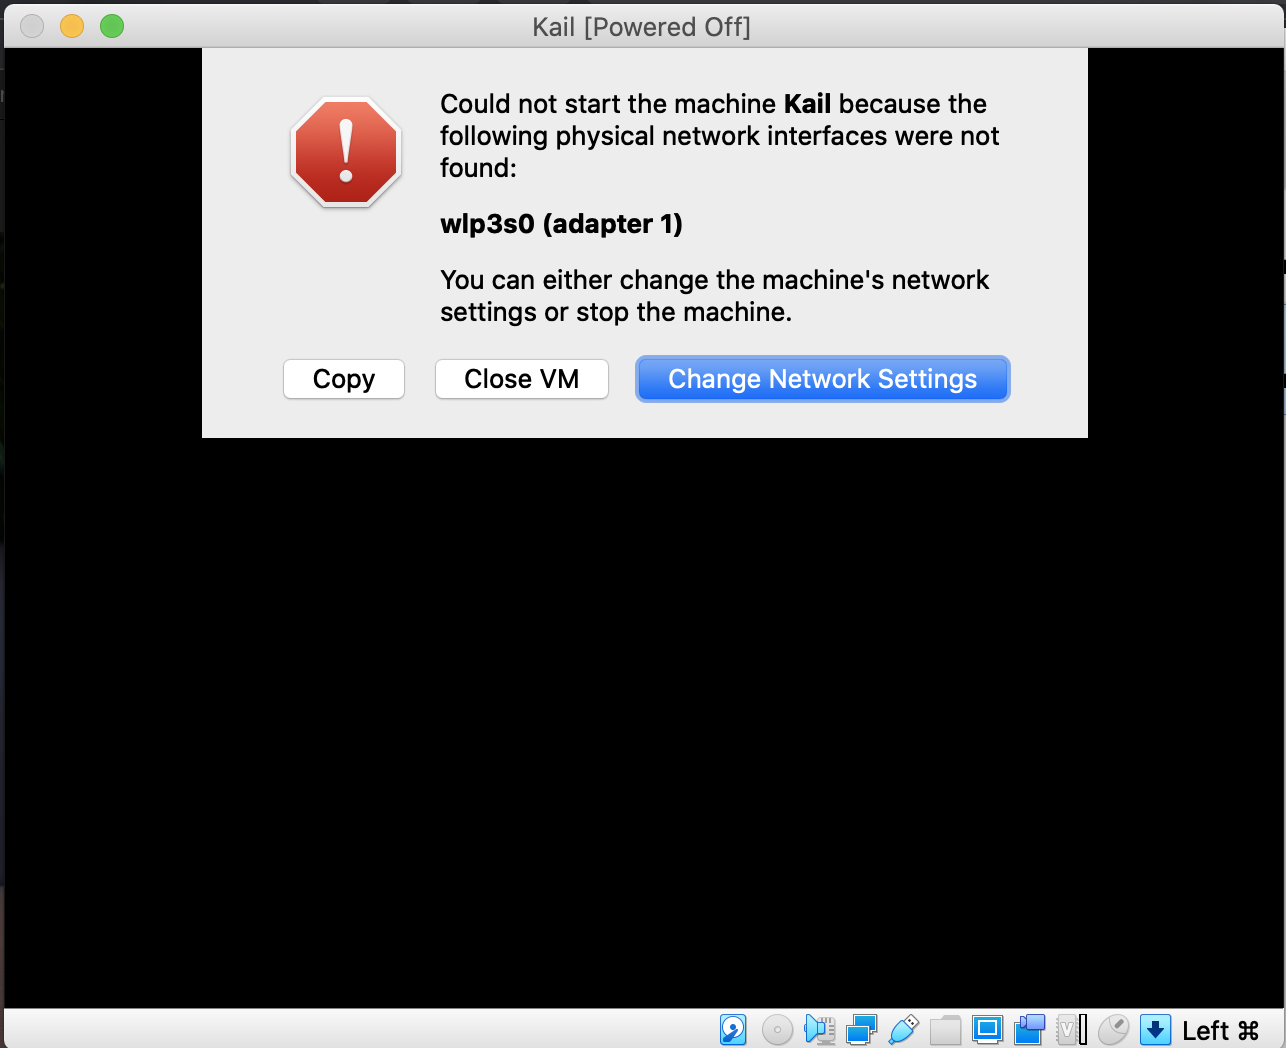
\includegraphics[scale=0.5]{Images/vm_error.png}
    \caption{The Bridged Connection Error}
    \label{fig:vmerror}
\end{figure}

The code seen in Listing \ref{code:bcn} is the Packer implementation of a VBoxManage command. This command tells the virtual machine to set the interface of the bridged adapter to \texttt{"en0"} which is the interface of my laptop. I do this before the virtual machine boots so this will change the adapter before the error can happen. The interface for the virtual machines can be specified in the config file.









